\section*{NAIL062 V\&P Logika: 10. sada příkladů -- Rezoluční metoda v PL}
% po 5. přednášce


\subsection*{Výukové cíle:} Po absolvování cvičení student

    \begin{itemize}\setlength{\itemsep}{0pt}
        \item rozumí pojmu unifikace, umí provádět Unifikační algoritmus
        \item zná potřebné pojmy z rezoluční metody v predikátové logice (rezoluční pravidlo, rezolventa, rezoluční důkaz/zamítnutí, rezoluční strom), umí je formálně definovat, uvést příklady, vysvětlit rozdíly oproti výrokové logice, 
        \item umí aplikovat rezoluční metodu k řešení daného problému (slovní úlohy, aj.), provést všechny potřebné kroky (převod do PNF, skolemizace, převod do CNF)
        \item umí sestrojit rezoluční zamítnutí dané (i nekonečné) CNF formule (existuje-li), a také nakreslit příslušný rezoluční strom, včetně uvedení použitých unifikací
        \item z rezolučního stromu umí sestrojit nesplnitelnou konjunkci základních instancí axiomů
        \item zná pojem LI-rezoluce, umí najít LI-zamítnutí dané teorie (existuje-li)
        \item seznámil se s vybranými pojmy z teorie modelů
    \end{itemize}
    

\section*{Příklady na cvičení}


\begin{problem} 
    
    Víme, že platí následující:
    \begin{itemize}\it
        \item Každý holič holí všechny, kdo neholí sami sebe
        \item Žádný holič neholí nikoho, kdo holí sám sebe.
    \end{itemize}
    Formalizujte ve vhodném jazyce predikátové logiky a dokažte rezolucí, že: {\it Neexistují žádní holiči.}

    \begin{solution}
                    
    \end{solution}
    
\end{problem}


\begin{problem}

    Mějme jazyk $L=\langle <, j, h, s\rangle$ bez rovností, kde $j,h,q$ jsou konstantní symboly značící (po řadě) jablka, hrušky, švestky, dále $<$ je binarní relační symbol a $x < y$ značí, že {\it ``ovoce $y$ je lepší než ovoce $x$''}. Víme, že:
    \begin{enumerate}[(i)]\it
        \item Relace ``být lepší'' je ostré částečné uspořádání (ireflexivní, asymetrická, tranzitivní relace).
        \item Hrušky jsou lepší než jablka.
    \end{enumerate}
    Chceme rezolucí dokázat následující tvrzení.
    \begin{enumerate}[(i))]\it
        \setcounter{enumi}{2}
        \item Jsou-li švestky lepší než hrušky, nejsou jablka lepší než švestky.
    \end{enumerate}
    Konkrétně:
    \begin{enumerate}[(a)]
    \item Tvrzení $(i)$, $(ii)$, $(iii)$ vyjádřete otevřenými formulemi jazyka $L$.
    \item Pomocí předchozích formulí či jejich negací nalezněte otevřenou teorii $T$ nad $L$ axiomatizovanou klauzulemi, která je nesplnitelná, právě když z $(i)$, $(ii)$ vyplývá $(iii)$. Napište $T$ v množinové reprezentaci.
    \item Rezolucí dokažte, že $T$ není splnitelná. Rezoluční zamítnutí znázorněte rezolučním stromem. U každého kroku uveďte použitou unifikaci. {\it Nápověda: stačí čtyři rezoluční kroky.}
    \item Nalezněte konjunkci základních instancí axiomů $T$, která je nesplnitelná. {\it Nápověda: využijte unifikace z (c).}
    \item Je $T$ zamítnutelná LI-rezolucí? Uveďte zdůvodnění.
    \end{enumerate}

    \begin{solution}
                    
    \end{solution}

\end{problem}


\begin{problem}

    Ukažte, že daná množina klauzulí je zamítnutelná (rezolucí). Popište zamítnutí pomocí rezolučního stromu. V každém kroku rezoluce napište použitou unifikaci a podtrhněte rezolvované literály.
    \begin{align*}
        S=\{
            &\{P(a,x,f(y)),P(a,z,f(h(b))),\neg Q(y,z)\},\\
            &\{\neg Q(h(b),w),H(w,a)\},\\
            &\{\neg P(a,w,f(h(b))),H(x,a)\},\\
            &\{P(a,u,f(h(u))),H(u,a),Q(h(b),b)\},\\
            &\{\neg H(v,a)\}
        \}
    \end{align*}

    \begin{solution}
                    
    \end{solution}

\end{problem}

        
        
\section*{Další příklady k procvičení}


\begin{problem}

    Jsou dána následující tvrzení o~proběhlém genetickém experimentu:
    \begin{enumerate}[(i)]\it
        \item Každá ovce byla buď porozena jinou ovcí, nebo byla naklonována (avšak nikoli oboje zároveň).
        \item Žádná naklonovaná ovce neporodila.
    \end{enumerate}
    Chceme ukázat rezolucí, že pak: {\it (iii) Pokud ovce porodila, byla sama porozena.} Konkrétně:
    \begin{enumerate}
        \item Uvedená tvrzení vyjádřete \underline{sentencemi} $\varphi_1$, $\varphi_2$, $\varphi_3$ v jazyce $L=\langle P,K\rangle$ bez rovnosti, kde $P$ je binární relační symbol, $K$ je unární relační symbol a $P(x,y)$, $K(x)$ značí, že \emph{``ovce $x$ porodila ovci $y$''} a \emph{``ovce $x$ byla naklonována''}.    
        \item S využitím Skolemizace těchto formulí nebo jejich negací sestrojte množinu klauzulí $S$ (může být ve větším jazyce), která je nesplnitelná, právě když  $\{\varphi_1, \varphi_2\} \models \varphi_3$. Zapište ji v množinové reprezentaci.
        \item Najděte rezoluční zamítnutí $S$, znázorněte je rezolučním stromem. U každého kroku uveďte použitou unifikaci.
    \end{enumerate}

\end{problem}


\begin{problem}

    Nechť $T=\{\neg(\exists x) R(x), (\exists x)(\forall y)(P(x,y)\to P(y,x)), (\forall x)((\exists y)(P(x,y)\wedge P(y,x))\to R(x)),$ $(\forall x)(\exists y)P(x,y)\}$ je teorie jazyka $L=\langle P,R\rangle$ bez rovnosti.

    \begin{enumerate}[(a)]
        \item Skolemizací nalezněte k $T$ otevřenou ekvisplnitelnou teorii $T'$ (nad vhodně rozšířeným jazykem).
        \item Převeďte $T'$ na ekvivalentní teorii $S$ v CNF. Zapište $S$ v množinové reprezentaci.
        \item Nalezněte rezoluční zamítnutí teorie $S$. U každého kroku uveďte použitou unifikaci.
        \item Nalezněte konjunkci základních instancí axiomů $S$, která je nesplnitelná.
        \item Má teorie $T$ jednoduchou kompletní extenzi? Uveďte zdůvodnění.
    \end{enumerate}

\end{problem}

        
\begin{problem}

    Uvažme následující graf:
    \begin{center}
        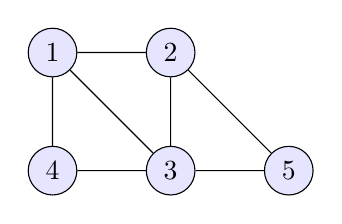
\begin{tikzpicture}[every node/.style={circle,fill=blue!10,draw,minimum size=0.5cm,node distance=1.5cm}]
            \node (1) {$1$};
            \node[right of=1] (2) {$2$};
            \node[below of=2] (3) {$3$};
            \node[left of=3] (4) {$4$};
            \path[draw] (1) -- (2) -- (3) -- (4) -- (1) -- (3);
            \node[right of=3] (5) {$5$};
            \path[draw] (2) -- (5) -- (3);
        \end{tikzpicture}
    \end{center}
    \begin{enumerate}[(a)]
        \item Najděte všechny automorfismy.
        \item Které podmnožiny množiny vrcholů $V$ jsou definovatelné? Uveďte definující formule. {\it (Nápověda: Využijte (a).)}
        \item Které binární relace na $V$ jsou definovatelné?
    \end{enumerate}    

\end{problem}


\begin{problem}

    Nechť $T=\{\varphi\}$ je teorie jazyka $L=\langle U, c \rangle$ s rovností, kde $U$ je unární relační symbol, $c$ je konstantní symbol a axiom $\varphi$ vyjadřuje \emph{``Existuje alespoň $5$ prvků, pro které platí U(x).''}
    \begin{enumerate}[(a)]
        \item Nalezněte dvě neekvivalentní jednoduché kompletní extenze teorie $T$ nebo zdůvodněte, proč neexistují.
        \item Je teorie $T$ otevřeně axiomatizovatelná? Uveďte zdůvodnění.
    \end{enumerate}

\end{problem}


\begin{problem}

    Nechť $T = \{U(x) \to U(f(x)), (\exists x)U(x), \neg (f(x) = x), \varphi\}$ je teorie v jazyce $L = \langle U, f \rangle$ s rovností, kde $U$ je unární relační symbol, $f$ je unární funkční symbol a $\varphi$ vyjadřuje, že ``existují maximálně 4 prvky''.
    \begin{enumerate}[(a)]
        \item Je teorie $T$ extenzí teorie $S = \{ (\exists x)(\exists y)(\neg x = y \land U(x) \land U(y)), \varphi \}$ v jazyce $L' = \langle U \rangle$? Je konzervativní extenzí? Zdůvodněte.
        \item Je teorie $T$ otevřeně axiomatizovatelná? Zdůvodněte.    
    \end{enumerate}
\end{problem}


\begin{problem}

    Buď $T=\{(\forall x)(\exists y) S(y)=x,\ S(x)=S(y)\to x=y\}$ teorie v~jazyce $L=\langle S\rangle$ s~rovností, kde $S$ je unární funkční symbol.
    \begin{enumerate}[(a)]
        \item Nalezněte extenzi $T'$ teorie $T$ o definici nového unárního funkčního symbolu $P$ takovou, že $T' \models S(S(x))=y \leftrightarrow P(P(y))=x$.
        \item Je teorie $T'$ otevřeně axiomatizovatelná? Uveďte zdůvodnění.
    \end{enumerate}

\end{problem} 


\section*{K zamyšlení}


\begin{problem}

    Nechť $T$ je extenze teorie $DeLO^-$ (tj. hustých lineárních uspořádání s minimálním prvkem a bez maximálního prvku) o nový axiom $c \le d$ v jazyce $L=\langle \le,c,d\rangle$ s rovností, kde $c$, $d$ jsou nové konstantní symboly.
    \begin{enumerate}[(a)]
        \item Jsou sentence $(\exists x)(x\le d \wedge x \ne d)$ a $(\forall x)(x \le d)$ pravdivé / lživé / nezávislé v $T$? Uveďte zdůvodnění.
        \item Napište dvě neekvivalentní jednoduché kompletní extenze teorie $T$.
    \end{enumerate}
    
\end{problem}


\begin{problem}

    Buď $T=\{(\forall x)(\exists y) S(y)=x,\ S(x)=S(y)\to x=y\}$ teorie v~jazyce $L=\langle S\rangle$ s~rovností, kde $S$ je unární funkční symbol.
    \begin{enumerate}[(a)]
        \item Buď $\mathcal{R}=\langle\mathbb{R},S\rangle$, kde $S(r)=r+1$ pro $r\in\mathbb{R}$. Právě pro která $r\in\mathbb{R}$ je množina $\{r\}$ definovatelná v~$\mathcal{R}$ z~parametru $0$?
        \item Je teorie $T$ otevřeně axiomatizovatelná? Uveďte zdůvodnění.
        \item Je extenze $T'$ teorie $T$ o~axiom $S(x)=x$ $\omega$-kategorická teorie? Je $T'$ kompletní?
        \item Pro která $0<n\in\mathbb{N}$ existuje $L$-struktura $\mathcal{B}$ velikosti $n$ elementárně ekvivalentní s~$\mathcal{R}$? Existuje spočetná struktura $\mathcal{B}$ elementárně ekvivalentní s~$\mathcal{R}$?
    \end{enumerate}

\end{problem}


\begin{problem}

    Známe následující informace o zadávání zakázek:
    \begin{enumerate}[(i)] \it
        \item Každý úředník, který je odpovědný za nějakou zakázku a vezme od nějaké společnosti úplatek, je kriminálník.
        \item Zakázku vyhraje pouze společnost, která podplatí všechny úředníky odpovědné za tuto zakázku.
        \item Pan Lubor je úředník.
        \item Nějaká společnost vyhrála nějakou zakázku, za kterou je pan Lubor odpovědný.
    \end{enumerate}
    Pomocí rezoluce dokažte, že: {\it (v) Pan Lubor je kriminálník.}
    \begin{enumerate}[(a)]
        \item Uvedená tvrzení vyjádřete \underline{sentencemi} $\varphi_1, \dots, \varphi_5$ v jazyce $L=\langle U, Z, S, K, P, V, O, l \rangle$ bez rovnosti, kde $U, Z, S$ a $K$ jsou unární relační symboly a $U(x), Z(x), S(x), K(x)$ znamenají (po řadě) ``$x$ je úředník / zakázka / společnost / kriminálník'', $P, V, O$ jsou binární relační symboly, kde $P(x,y), V(x,y), O(x,y)$ značí (po řadě) ``$x$ podplatil $y$'', ``$x$ vyhrál $y$'' a ``$x$ je odpovědný za $y$'' a $l$ je konstanta označující pana Lubora.
        \item Pomocí skolemizace předchozích formulí nalezněte otevřenou teorii $T$ (případně ve větším jazyce), která je nesplnitelná, právě když  $\{\varphi_1, \varphi_2, \varphi_3, \varphi_4\} \models \varphi_5$.
        \item Převedením axiomů $T$ do CNF nalezněte teorii $T'$ ekvivalentní $T$ a axiomatizovanou klauzulemi. Napište $T'$ v množinové reprezentaci.
        \item Rezolucí dokažte, že $T'$ není splnitelná. Rezoluční zamítnutí znázorněte rezolučním stromem. U každého kroku uveďte použitou unifikaci.
        \item Nalezněte konjunkci základních instancí axiomů $T'$, která je nesplnitelná.
    \end{enumerate}

\end{problem}

\end{document}


